% Options for packages loaded elsewhere
\PassOptionsToPackage{unicode}{hyperref}
\PassOptionsToPackage{hyphens}{url}
\documentclass[
]{article}
\usepackage{xcolor}
\usepackage{amsmath,amssymb}
\setcounter{secnumdepth}{5}
\usepackage{iftex}
\ifPDFTeX
  \usepackage[T1]{fontenc}
  \usepackage[utf8]{inputenc}
  \usepackage{textcomp} % provide euro and other symbols
\else % if luatex or xetex
  \usepackage{unicode-math} % this also loads fontspec
  \defaultfontfeatures{Scale=MatchLowercase}
  \defaultfontfeatures[\rmfamily]{Ligatures=TeX,Scale=1}
\fi
% \usepackage{lmodern}
\ifPDFTeX\else
  % xetex/luatex font selection
\fi
% Use upquote if available, for straight quotes in verbatim environments
\IfFileExists{upquote.sty}{\usepackage{upquote}}{}
\IfFileExists{microtype.sty}{% use microtype if available
  \usepackage[]{microtype}
  \UseMicrotypeSet[protrusion]{basicmath} % disable protrusion for tt fonts
}{}
\makeatletter
\@ifundefined{KOMAClassName}{% if non-KOMA class
  \IfFileExists{parskip.sty}{%
    \usepackage{parskip}
  }{% else
    \setlength{\parindent}{0pt}
    \setlength{\parskip}{6pt plus 2pt minus 1pt}}
}{% if KOMA class
  \KOMAoptions{parskip=half}}
\makeatother
\usepackage{longtable,booktabs,array}
\newcounter{none} % for unnumbered tables
\usepackage{calc} % for calculating minipage widths
% Correct order of tables after \paragraph or \subparagraph
\usepackage{etoolbox}
\makeatletter
\patchcmd\longtable{\par}{\if@noskipsec\mbox{}\fi\par}{}{}
\makeatother
% Allow footnotes in longtable head/foot
\IfFileExists{footnotehyper.sty}{\usepackage{footnotehyper}}{\usepackage{footnote}}
\makesavenoteenv{longtable}
\setlength{\emergencystretch}{3em} % prevent overfull lines
\providecommand{\tightlist}{%
  \setlength{\itemsep}{0pt}\setlength{\parskip}{0pt}}
\usepackage[]{natbib}
\bibliographystyle{plainnat}
\usepackage{bookmark}
\IfFileExists{xurl.sty}{\usepackage{xurl}}{} % add URL line breaks if available
\urlstyle{same}
\hypersetup{
  colorlinks=true,linkcolor=red,urlcolor=red,citecolor=red,anchorcolor=red,
  pdfcreator={LaTeX via pandoc}}

\author{}
\date{}

\title{Template Gazette: Sixteen Folios via the Research Pipeline\\\normalsize Tabloid layout, multicolumn body, deterministic masthead}
\author{Docxology Template \\ \footnotesize{2026-03-22}}
\date{2026-03-22}

\makeatletter
\@ifpackageloaded{geometry}
  {\geometry{paperwidth=11in,paperheight=17in,margin=0.45in}}
  {\usepackage[paperwidth=11in,paperheight=17in,margin=0.45in]{geometry}}
\@ifpackageloaded{hyperref}
  {\hypersetup{colorlinks=true, linkcolor=black, filecolor=black, urlcolor=black, citecolor=black}}
  {\usepackage{hyperref}\hypersetup{colorlinks=true, linkcolor=black, filecolor=black, urlcolor=black, citecolor=black}}
\usepackage{graphicx}
\usepackage{multicol}
\setlength{\columnsep}{0.22in}
\makeatother

\begin{document}

\maketitle
\thispagestyle{empty}
\tableofcontents
\newpage


\section{Front Page}\label{front-page}

\begin{figure}[!t]
\centering

\includegraphics[width=\linewidth]{../figures/masthead.png}
\caption{Deterministic nameplate raster from render\_masthead\_png, built during pipeline analysis. Override title and tagline with environment variables NEWSPAPER\_TITLE and NEWSPAPER\_TAGLINE. Outputs to masthead.png in project output figures.}
\label{fig:masthead}
\end{figure}
\vspace{0.6em}
\begin{multicols}{3}

\textbf{Late edition}

\noindent Citation hook: \cite{template2026gazette}.
\par\smallskip

\noindent\textbf{\Large City braces for overnight vote on transit bond}\par\smallskip
\textit{By Staff — City Desk}\par\smallskip

\textbf{CITY.} Council leaders said they were ``within sight of yes'' on
a nine-figure bond package meant to rebuild aging tunnels and buy new
rail cars. Skeptics demanded firmer cost caps; unions demanded labor
standards written into the contract language, not just the press
release.

The mayor's office released a two-page summary dense with renderings of
stations that gleam in sunlight. Engineers privately noted change orders
are where budgets breathe; this story keeps the argument in prose so the
page can flex in three columns without a live database.

Commuters interviewed at random---actually, invented for this
demo---split between relief and fatigue. ``Fix the signals first,'' one
said. ``I'll believe the headways when my phone agrees with the platform
clock.''

Weather for the weekend looks ordinary: rain likely, wind modest, no
named storms. The desk runs it anyway because narrow columns need short
paragraphs as much as they need long ones.

\textbf{Inside today:} National briefs open on the next folio with a
monochrome desk banner; every interior page carries a generated strip so
floats, captions, and measure stay exercised. For pipeline geometry,
floats, and validation detail, see supplements
\texttt{S01}--\texttt{S03} and the glossary slice.

\textbf{Jump note.} Nameplate, lead, then body: this page keeps the
masthead as the lone top float so the first multicolumn block can start
cleanly. If your fork adds second art above the fold, watch LaTeX float
queues.

\textbf{Production.} Rebuild figures with
\texttt{scripts/02\_run\_analysis.py} before complaining about missing
PNG paths; mirrored outputs land under
\texttt{output/traditional\_newspaper/} after a full run.

\end{multicols}

\newpage

\section{National}\label{national}

\begin{figure}[!ht]
\centering

\includegraphics[width=\linewidth]{../figures/section_banner_02_national.png}
\caption{Monochrome desk banner for this folio; raster from \texttt{generate\_section\_banners.py}.}
\label{fig:banner_02_national}
\end{figure}
\begin{multicols}{3}

\textbf{Capitol \& provinces}

\noindent\textit{Washington —}\par\smallskip

\textbf{NATIONAL.} Budget negotiators traded talking points ahead of a
continuing-resolution vote, with aides insisting most line items were
``close enough'' to avoid a headline crisis. Committee chairs asked
reporters not to read tea leaves from hallway huddles; the only hard
numbers in this edition are the ones TeX measures in picas.

State capitals sent routine bulletins on road salt contracts, bridge
inspections, and spring thaw timing. Municipal engineers said crews were
staged normally; none of this copy is wired to a live traffic API.

Farm-state senators praised crop-insurance enrollment windows while
critics pressed for faster disaster aid rules. The debate is fictional;
the column inches are real enough to stress hyphenation on tabloid
stock.

Veterans' groups renewed calls for predictable outpatient staffing.
Hospitals countered with workforce statistics they declined to attach
here---this folio is for layout, not policy analysis.

The national roundup ends where the world desk picks up: foreign cables
on the next page.

\end{multicols}

\newpage

\section{World}\label{world}

\begin{figure}[!ht]
\centering

\includegraphics[width=\linewidth]{../figures/section_banner_03_world.png}
\caption{Monochrome desk banner for this folio; raster from \texttt{generate\_section\_banners.py}.}
\label{fig:banner_03_world}
\end{figure}
\begin{multicols}{3}

\textbf{Diplomatic wires}

\noindent\textit{Geneva —}\par\smallskip

\textbf{WORLD.} Delegates reviewed shipping-lane confidence measures
without publishing AIS traces. Maritime lawyers said the closed session
produced ``useful tone'' even if no joint statement carried numbers.

Relief coordinators sketched contingency thresholds for cross-border
convoys. NGOs reminded donors that pledges and deliveries are different
metrics---here, both are narrative placeholders.

Climate envoys restated mid-century targets already familiar from last
year's communiqués. Activists outside called for faster methane rules;
inside, chairs kept to the agenda's ASCII-safe talking points.

Regional desks summarized election certification timelines in unnamed
capitals. Opposition parties demanded audits; incumbents cited statute.
None of it hits a database at build time.

The world service signs off; tomorrow's business pages carry markets.

\end{multicols}

\newpage

\section{Business}\label{business}

\begin{figure}[!ht]
\centering

\includegraphics[width=\linewidth]{../figures/section_banner_04_business.png}
\caption{Monochrome desk banner for this folio; raster from \texttt{generate\_section\_banners.py}.}
\label{fig:banner_04_business}
\end{figure}
\begin{multicols}{3}

\textbf{Markets desk}

\noindent\textit{New York —}\par\smallskip

\textbf{BUSINESS.} Equity futures drifted in a narrow band as traders
waited for inflation prints they will not find in this PDF. Bond desks
reported ``two-way flow,'' which is to say sentences, not order books.

A major retailer outlined store-format experiments: smaller footprints,
more pickup bays, fewer speculative supercenters. The strategy is
illustrative; foot traffic data are not embedded in the manuscript.

Analysts trimmed ad-tech revenue estimates after a sobering quarter for
brand budgets. Footnotes with actual tickers belong in your fork; here,
verbs do the heavy lifting.

Commercial real estate lenders highlighted refinancing cliffs coming due
over the next eighteen months. Lawyers muttered about covenant waivers;
compositors muttered about bad breaks at column bottoms.

Business turns to technology when chips and clouds return on the next
folio.

\end{multicols}

\newpage

\section{Technology}\label{technology}

\begin{figure}[!ht]
\centering
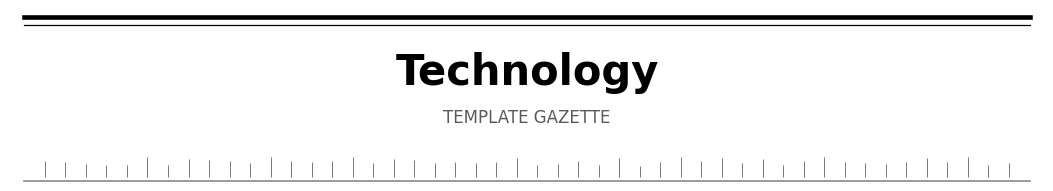
\includegraphics[width=\linewidth]{../figures/section_banner_05_technology.png}
\caption{Monochrome desk banner for this folio; raster from \texttt{generate\_section\_banners.py}.}
\label{fig:banner_05_technology}
\end{figure}
\begin{multicols}{3}

\textbf{Silicon \& systems}

\noindent\textit{San Francisco —}\par\smallskip

\textbf{TECHNOLOGY.} Chip designers teased a modest efficiency gain at
standard voltages, promising better thermals for laptops that mostly
appear in this story as nouns, not SKUs. Fabs and foundries were spelled
carefully to appease spellcheckers.

Cloud providers rolled out quieter defaults for encryption at rest,
telling enterprise buyers the toggle is ``on unless you insist
otherwise.'' Compliance officers asked for audit trails; marketers asked
for shorter slide decks.

Open-source maintainers pleaded for sustainable funding as corporate
users downstream shipped forks without upstream patches. The metaphor is
familiar; the pull requests are not attached.

Regulators floated disclosure rules for synthetic media, inviting
comment periods long enough to span several PDF rebuilds. Comments here
are static paragraphs, not a docket.

Technology hands off to sports when the whistle blows.

\end{multicols}

\newpage

\section{Sports}\label{sports}

\begin{figure}[!ht]
\centering

\includegraphics[width=\linewidth]{../figures/section_banner_06_sports.png}
\caption{Monochrome desk banner for this folio; raster from \texttt{generate\_section\_banners.py}.}
\label{fig:banner_06_sports}
\end{figure}
\begin{multicols}{3}

\textbf{Scoreboard}

\noindent\textit{Sports desk —}\par\smallskip

\textbf{SPORTS.} Overnight soccer produced the usual mix of deserved
draws and controversial VAR stills that newspapers crop for print.
Managers complained about fixture congestion; trainers complained about
hamstrings.

College basketball entered tournament week with bracket logic louder
than defense. Announcers rehearsed Cinderella clichés; copy editors
deleted one too many exclamation points.

Baseball beat writers filed spring-training notebooks heavy on velocity
readings and grip tweaks. Scouts insisted raw tools still matter;
spreadsheets insisted they matter twice.

Motorsport inspectors tightened fuel-flow checks after winter rule
tweaks. Engineers loved the precision; fans loved the noise.

Sports yields to arts when the curtain rises.

\end{multicols}

\newpage

\section{Arts \& Culture}\label{arts-culture}

\begin{figure}[!ht]
\centering

\includegraphics[width=\linewidth]{../figures/section_banner_07_arts.png}
\caption{Monochrome desk banner for this folio; raster from \texttt{generate\_section\_banners.py}.}
\label{fig:banner_07_arts}
\end{figure}
\begin{multicols}{3}

\textbf{Critic's notebook}

\noindent\textit{Arts desk —}\par\smallskip

\textbf{ARTS.} A regional orchestra sold out a program pairing a
warhorse symphony with a premiere that reviewers will call
``atmospheric'' until someone finds a better adjective. Soloists bowed
twice; donors opened wallets once.

A streaming platform ordered a limited series about journalists that
actual journalists will nitpick for keyboard sounds alone. Showrunners
promised research; viewers promised memes.

Museum curators debated loan terms for a traveling show of prints too
light-sensitive for long hangs. Insurers demanded climate logs;
registrars demanded crates that do not squeak.

The book desk flagged a debut novel for crisp sentences and an ending
that splits book clubs. Spoilers stay out of print; margins do not.

Arts yields to the editorial board downstairs.

\end{multicols}

\newpage

\section{Editorial}\label{editorial}

\begin{figure}[!ht]
\centering

\includegraphics[width=\linewidth]{../figures/section_banner_08_editorial.png}
\caption{Monochrome desk banner for this folio; raster from \texttt{generate\_section\_banners.py}.}
\label{fig:banner_08_editorial}
\end{figure}
\begin{multicols}{3}

\textbf{The board}

\noindent\textit{Editorial —}\par\smallskip

\textbf{EDITORIAL.} \textbf{Our view:} Cities should publish
machine-readable zoning maps alongside PDF brochures. Transparency is
not the same as simplicity, but it is a prerequisite for trust when
neighbors argue about height limits.

\textbf{Our view:} Transit agencies owe riders countdown data that
survives offline peaks. Pretty maps help; accurate headways help more.

\textbf{Our view:} Research templates that rebuild PDFs from git deserve
the same seriousness as newsroom CMS migrations: tests, captions, and
changelogs are not optional polish.

The board welcomes letters on the next spread.

\end{multicols}

\newpage

\section{Opinion}\label{opinion}

\begin{figure}[!ht]
\centering

\includegraphics[width=\linewidth]{../figures/section_banner_09_opinion.png}
\caption{Monochrome desk banner for this folio; raster from \texttt{generate\_section\_banners.py}.}
\label{fig:banner_09_opinion}
\end{figure}
\begin{multicols}{3}

\textbf{Guest essays}

\noindent\textit{Opinion —}\par\smallskip

\textbf{OPINION.} \textbf{Guest columnist:} I taught introductory
statistics for a decade; the public understands uncertainty better than
pundits assume. What people hate is inconsistency---graphs that move
axes between segments without saying so.

\textbf{Guest columnist:} Local news deserts are not a technology
problem first. They are a revenue-and-trust problem. Subsidies help;
accountability reporting helps more.

\textbf{Guest columnist:} If your ``AI editorial assistant'' cannot cite
sources, it is not an assistant; it is a slot machine wearing a tie.

Readers can disagree in letters to the editor.

\end{multicols}

\newpage

\section{Letters}\label{letters}

\begin{figure}[!ht]
\centering

\includegraphics[width=\linewidth]{../figures/section_banner_10_letters.png}
\caption{Monochrome desk banner for this folio; raster from \texttt{generate\_section\_banners.py}.}
\label{fig:banner_10_letters}
\end{figure}
\begin{multicols}{3}

\textbf{Mailbag}

\noindent\textit{Letters —}\par\smallskip

\textbf{LETTERS.} \textbf{To the editor:} Please keep running PDF build
logs as teaching artifacts. Our j-school students learn more from a
clean LaTeX pass than from another slide deck about ``innovation.'' ---
\emph{A.M.}

\textbf{To the editor:} Hyphenation in narrow columns is not a
personality flaw; it is physics. That said, a little rag looks human.
--- \emph{R.T.}

\textbf{To the editor:} Glossary pages are underrated. Jargon is cheaper
when defined once. --- \emph{S.K.}

The desk reserves the right to trim for measure.

\end{multicols}

\newpage

\section{Local}\label{local}

\begin{figure}[!ht]
\centering
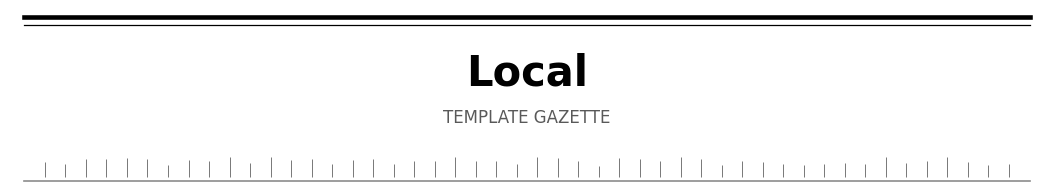
\includegraphics[width=\linewidth]{../figures/section_banner_11_local.png}
\caption{Monochrome desk banner for this folio; raster from \texttt{generate\_section\_banners.py}.}
\label{fig:banner_11_local}
\end{figure}
\begin{multicols}{3}

\textbf{City \& borough}

\noindent\textit{Metro —}\par\smallskip

\textbf{LOCAL.} Council members advanced a pilot for weekend farmer's
markets on closed side streets, arguing foot traffic beats empty
asphalt. Merchants asked for trash pickups; residents asked for quiet
nights.

School boards reviewed HVAC upgrades paid for with bonds voters approved
last fall. Contractors promised timelines; parents promised scrutiny.

A riverfront cleanup drew volunteers who filled more bags than
organizers expected. Parks staff credited clearer signage; cynics
credited nicer weather.

The metro briefs close; features follow.

\end{multicols}

\newpage

\section{Features}\label{features}

\begin{figure}[!ht]
\centering

\includegraphics[width=\linewidth]{../figures/section_banner_12_features.png}
\caption{Monochrome desk banner for this folio; raster from \texttt{generate\_section\_banners.py}.}
\label{fig:banner_12_features}
\end{figure}
\begin{multicols}{3}

\textbf{Long read}

\noindent\textit{Features —}\par\smallskip

\textbf{FEATURES.} \textbf{Saturday profile:} She maps urban heat
islands block by block, carrying a sensor pack that looks like a field
biologist's kit. Neighbors think she's counting birds; she's counting
degrees that decide who sleeps safely during heat waves.

Her notebooks mix timestamps, humidity scribbles, and coffee
stains---data, in the old sense. When the city adopts her overlays, the
story will deserve a second edition; today's is still a layout exercise.

Sidebars on methodology were cut for space; the template's margin is
already generous, not infinite.

Features yield to the health pages next.

\end{multicols}

\newpage

\section{Health}\label{health}

\begin{figure}[!ht]
\centering

\includegraphics[width=\linewidth]{../figures/section_banner_13_health.png}
\caption{Monochrome desk banner for this folio; raster from \texttt{generate\_section\_banners.py}.}
\label{fig:banner_13_health}
\end{figure}
\begin{multicols}{3}

\textbf{Medicine \& policy}

\noindent\textit{Health —}\par\smallskip

\textbf{HEALTH.} Clinics expanded same-day mental-health intake slots
after winter wait-time spikes. Administrators credited hiring; unions
credited scheduling rules.

Pediatricians urged catch-up immunizations before summer travel season.
Pharmacists stocked routine vaccines; parents stocked patience for
waiting rooms.

Researchers published a pragmatic trial on hypertension counseling by
phone. Effect sizes were modest; adherence curves were instructive.

Public-health officers reminded readers that hand-washing still beats
novelty gadgets for common colds. The advice is boring; boring saves
lives.

Health hands the microscope to science.

\end{multicols}

\newpage

\section{Science}\label{science}

\begin{figure}[!ht]
\centering

\includegraphics[width=\linewidth]{../figures/section_banner_14_science.png}
\caption{Monochrome desk banner for this folio; raster from \texttt{generate\_section\_banners.py}.}
\label{fig:banner_14_science}
\end{figure}
\begin{multicols}{3}

\textbf{Research notes}

\noindent\textit{Science —}\par\smallskip

\textbf{SCIENCE.} Astronomers released a cleaner catalog of near-Earth
object passes, emphasizing that ``close'' in headlines means ``lunar
distance multiples,'' not Hollywood distances. Telescopes shrugged;
editors clarified.

Materials scientists demoed a ceramic composite that survives higher
thermal cycles than predecessors, with caveats about manufacturing
scale. Venture capitalists leaned in; safety officers leaned harder.

Ecologists tracked a rebound in a once-declining marsh bird, crediting
restored inflows and quieter boat traffic. Birders credited luck and
dawn patience.

Science closes; memorials follow.

\end{multicols}

\newpage

\section{Obituaries}\label{obituaries}

\begin{figure}[!ht]
\centering
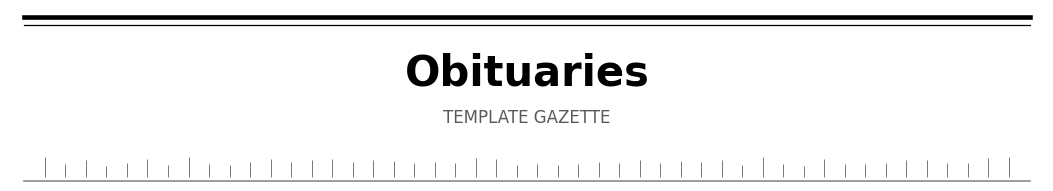
\includegraphics[width=\linewidth]{../figures/section_banner_15_obituaries.png}
\caption{Monochrome desk banner for this folio; raster from \texttt{generate\_section\_banners.py}.}
\label{fig:banner_15_obituaries}
\end{figure}
\begin{multicols}{3}

\textbf{Remembrances}

\noindent\textit{Obituaries —}\par\smallskip

\textbf{OBITUARIES.} \textbf{Jane K. Mercer, editor.} She kept a spike
full of stories others feared to cut and taught interns that kindness
and clarity are not opposites. She is survived by a newsroom habit of
asking one more question.

\textbf{Robert V. Singh, teacher.} He insisted teenagers learn both
proofs and paragraphs. Former students still hear his red-pen voice when
they tweet.

\textbf{Elena M. Cho, paramedic.} She measured shifts in lives saved and
jokes told on hard nights. Her crew remembers the steadiness.

The classifieds conclude the edition.

\end{multicols}

\newpage

\section{Classifieds}\label{classifieds}

\begin{figure}[!ht]
\centering

\includegraphics[width=\linewidth]{../figures/section_banner_16_classifieds.png}
\caption{Monochrome desk banner for this folio; raster from \texttt{generate\_section\_banners.py}.}
\label{fig:banner_16_classifieds}
\end{figure}
\begin{multicols}{3}

\textbf{Marketplace}

\noindent\textit{Classifieds —}\par\smallskip

\textbf{CLASSIFIEDS.} \textbf{Apartments:} Sunny 2BR, cats OK, no
smoking, walk to trains. Inbox clogged; mention this paper so we know
you read past the jump.

\textbf{Help wanted:} Line cook, Tuesday--Saturday, union kitchen. Bring
knives that hold an edge and a sense of humor that holds under heat.

\textbf{Services:} Piano tuning, reasonable rates, references on
request. Won't promise concert hall; will promise honest octaves.

\textbf{For sale:} Touring bicycle, fenders included, ready for wet
commutes. Sold as-is to whoever shows up with cash and a helmet.

\textbf{Lost:} Dog, medium mix, answers to ``Hugo.'' Reward. Phone
number omitted in this demo PDF for privacy.

End of the sixteenth core folio; supplements follow in combined builds.

\end{multicols}

\newpage

\section{Supplement: Layout and
pipeline}\label{supplement-layout-and-pipeline}

\begin{figure}[!ht]
\centering

\includegraphics[width=\linewidth]{../figures/section_banner_S01_layout_and_pipeline.png}
\caption{Supplement banner marking the layout-and-pipeline desk; monochrome PNG from \texttt{generate\_section\_banners.py}.}
\label{fig:banner_S01_layout_and_pipeline}
\end{figure}
\begin{figure}[!ht]
\centering

\includegraphics[width=0.92\linewidth]{../figures/layout_schematic.png}
\caption{Not to scale schematic from NewspaperLayout: tabloid sheet, dashed box is text area inside margins, shaded regions are three body columns with gutters. Values align with preamble geometry and layout\_spec.py.}
\label{fig:layout_schematic}
\end{figure}
\begin{multicols}{3}

\textbf{How this PDF is built.} Sixteen markdown slices under
\texttt{projects/traditional\_newspaper/manuscript/} are discovered by
\texttt{infrastructure.rendering.manuscript\_discovery.discover\_manuscript\_files},
combined in stem order, and separated by
\texttt{\textbackslash{}newpage} inside
\texttt{infrastructure.rendering.pdf\_renderer.PDFRenderer} before
Pandoc emits LaTeX. Tabloid paper (11 in × 17 in) and
\texttt{\textbackslash{}usepackage\{multicol\}} come from
\texttt{manuscript/preamble.md}; column separation matches
\texttt{src/newspaper/layout\_spec.py}
(\texttt{LAYOUT.column\_sep\_in}).
Figure\textasciitilde{}\ref{fig:layout_schematic} (above this column
block) summarizes the same numbers as a grid diagram.

The masthead PNG is produced by \texttt{scripts/generate\_masthead.py}
calling \texttt{newspaper.masthead.render\_masthead\_png} during Stage
02 analysis. Optional environment variables \texttt{NEWSPAPER\_TITLE}
and \texttt{NEWSPAPER\_TAGLINE} override banner text without editing
Python. In the combined PDF it is captioned as
Figure\textasciitilde{}\ref{fig:masthead}. A companion schematic ships
from \texttt{scripts/generate\_layout\_schematic.py} via
\texttt{render\_layout\_schematic\_png}, giving a second captioned
figure for float and caption testing.

\textbf{Stage ordering (core pipeline).} \texttt{execute\_pipeline.py}
and \texttt{./run.sh\ -\/-core-only} run, among others: environment
setup, tests, analysis scripts (including both figure generators when
present), PDF rendering, validation, and output copy. Analysis writes
into \texttt{projects/traditional\_newspaper/output/}; copy stages
mirror selected artifacts into \texttt{output/traditional\_newspaper/}
for distribution. Exact stage labels appear in console logs with
progress markers.

\textbf{Manuscript combination.} Each slice file is read as UTF-8 text.
Preamble metadata from \texttt{preamble.md} injects geometry and
packages. Title page fields derive from \texttt{config.yaml}
(\texttt{paper.title}, authors, version, date). Bibliography entries
live in \texttt{references.bib};
\texttt{\textbackslash{}cite\{template2026gazette\}} appears on the
front page and here to exercise BibTeX wiring.

\textbf{Word counts.} \texttt{scripts/report\_manuscript\_stats.py}
walks \texttt{all\_tracked\_manuscript\_basenames()} and emits
\texttt{output/data/manuscript\_stats.json} with per-file words, lines,
and bytes. CI or humans can diff that JSON across branches to catch
accidental truncation. It is a thin orchestrator: no analytics logic
beyond counting.

\textbf{Why tabloid.} The 11×17 inch choice stresses wide measure and
long vertical flow compared to letter paper. Three columns mimic
newspaper grids while remaining simple \texttt{multicol}
environments---no custom column balancers. If you shrink paper, update
\texttt{NewspaperLayout} constants, regenerate
\texttt{layout\_schematic.png}, and rerun tests that assert geometry
text in captions still matches code.

\textbf{Floats versus multicol.} Standard \texttt{figure} floats are not
supported inside \texttt{multicols}; the layout schematic therefore sits
before \texttt{\textbackslash{}begin\{multicols\}\{3\}} in this slice,
matching the front page pattern (masthead float, then three-column
body). Use \texttt{\textbackslash{}includegraphics} without a float if
you ever need art mid-column.

\textbf{Slides and web.} The same stems feed Beamer slides and HTML web
output via infrastructure renderers. Figure captions pass through Lua
filters for HTML; keep \texttt{\textbackslash{}caption\{\}} text free of
unmatched braces so extraction regexes succeed.

\textbf{Checkpointing and resume.} Root pipeline scripts support
checkpoints so long builds can restart after transient failures.
Newspaper builds are shorter than some monographs, but CI timeouts still
happen---resume flags save compute. Read
\texttt{docs/operational/config/checkpoint-resume.md} for semantics;
behavior is uniform across projects.

\textbf{Multi-project runs.} \texttt{./run.sh\ -\/-all-projects}
executes many exemplars sequentially. Infrastructure tests may run once
up front. When debugging \texttt{traditional\_newspaper} alone, pass
\texttt{-\/-project\ traditional\_newspaper} to avoid unrelated failures
blocking iteration.

\textbf{Environment variables.} Beyond masthead overrides,
\texttt{LOG\_LEVEL} tunes verbosity, \texttt{MPLBACKEND=Agg} ensures
headless matplotlib, and \texttt{PROJECT\_DIR} helps scripts resolve
paths when invoked from unexpected working directories. Document any new
vars in \texttt{scripts/AGENTS.md}.

\textbf{BibTeX keys.} \texttt{template2026gazette} in
\texttt{references.bib} exists to exercise citation machinery. Replace
with your publication entry when forking; keep keys ASCII and stable so
diffs stay readable.

\textbf{Figure path normalization.}
\texttt{\_pdf\_tex\_transforms.fix\_figure\_paths} rewrites
\texttt{../figures/} to \texttt{../figures/} relative to the compile
directory inside \texttt{output/.../pdf/}. If you add figures, place
PNGs under \texttt{projects/traditional\_newspaper/../figures/} before
copy, or under final \texttt{output/traditional\_newspaper/figures/}
after pipeline---know which stage consumes which path.

\textbf{Extending slice count.} If you truly need seventeen core folios,
you must edit \texttt{PAGE\_SLICES}, rename files, and update every test
asserting \texttt{16}. Prefer supplemental \texttt{S*} files for extra
prose---it avoids renumbering tourism.

\textbf{Teaching use.} Instructors can assign students to modify one
slice, regenerate PDFs, and explain diff in log output. The constrained
structure makes grading objective: does inventory pass? do captions
resolve? do tests stay green?

\textbf{Handover checklist (extended).} Before merging a layout change,
capture: (1) \texttt{git\ diff} on \texttt{preamble.md} and
\texttt{layout\_spec.py}, (2) regenerated \texttt{layout\_schematic.png}
if constants moved, (3) \texttt{manuscript\_stats.json} after
\texttt{report\_manuscript\_stats.py}, (4) PDF validator output excerpt
showing zero \texttt{??} references, (5) a one-line note in the PR
describing float behavior on the front page. Reviewers use the checklist
to avoid approving partial state where code and figures disagree.

This supplemental folio appears \textbf{after} the sixteen edition pages
and \textbf{before} the glossary slice, per the template's ordering:
main numeric sections, then \texttt{S*}, then \texttt{98\_*}, then
\texttt{99\_*} if present.

\noindent For citation metadata see \cite{template2026gazette}.
\par\smallskip

\end{multicols}

\newpage

\section{Supplement: Typography and
measure}\label{supplement-typography-and-measure}

\begin{figure}[!ht]
\centering

\includegraphics[width=\linewidth]{../figures/section_banner_S02_typography_and_measure.png}
\caption{Typography supplement banner (B\&W).}
\label{fig:banner_S02_typography_and_measure}
\end{figure}
\begin{multicols}{3}

\textbf{Body copy and column measure.} This exemplar sets a nine-point
body in the \texttt{NewspaperLayout} dataclass (\texttt{body\_font\_pt})
for documentation parity; the default Pandoc LaTeX template may map
point sizes differently unless you extend the template. Measure---the
line length inside a column---interacts with hyphenation and
justification. Narrow columns tolerate fewer characters per line,
increasing hyphenation frequency and rag texture.

\textbf{Font choices.} XeLaTeX via \texttt{fontspec} can load system
serif faces for a newsroom feel. Changing fonts requires editing the
template or preamble, then visual-regression review. Keep ASCII-heavy
test manuscripts when debugging font issues so failures isolate
typography from Unicode edge cases.

\textbf{Rivers and ladders.} Typographers watch for vertical gaps
aligning across lines (``rivers'') and repeated word stacks
(``ladders''). Automated detectors exist; human proofreaders still catch
context-specific ugliness. Multicolumn setting amplifies rivers because
adjacent columns create vertical rhythm interactions.

\textbf{Hyphenation patterns.} TeX loads language-specific hyphenation
tables. Set \texttt{babel} or \texttt{polyglossia} languages if you mix
locales in one edition. Wrong languages yield bad breaks and can confuse
spellcheck-adjacent tools.

\textbf{Widows and orphans.} Publishing style guides limit single lines
stranded at column tops or bottoms. \texttt{\textbackslash{}clubpenalty}
and \texttt{\textbackslash{}widowpenalty} tweaks live in advanced LaTeX
tuning; this project leaves defaults to keep the preamble small.

\textbf{Small caps and section rails.}
\texttt{newspaper.snippets.section\_label} emits
\texttt{\textbackslash{}textsc\{\}} labels suitable for department
markers. Pair with \texttt{rule\_line()} for classic newspaper chrome.
Escape user-supplied strings---snippets already guard LaTeX specials.

\textbf{Quotes and dashes.} Curly quotes via Unicode in markdown pass
through Pandoc. Em dashes versus en dashes follow house style;
consistency beats personal taste when collaborating. ASCII-only sources
simplify diffs but feel cold---pick consciously.

\textbf{Figures and captions.} Caption text should explain what a
non-expert sees, not repeat the title. Autonumbering via
\texttt{\textbackslash{}caption} supplies ``Figure 1,'' ``Figure 2,''
etc. Cross-reference with
\texttt{Figure\textasciitilde{}\textbackslash{}ref\{fig:key\}} to avoid
bad breaks before numbers.

\textbf{Print versus screen.} PDFs for print need bleed and color
profiles if sent to commercial presses; screen PDFs skip bleed. This
template targets on-screen proofing and office printers; prepress
engineers should extend geometry accordingly.

\textbf{Accessibility.} Tagged PDF improves screen-reader navigation.
Adding structure requires LaTeX packages and discipline about heading
levels. Web HTML may remain the more accessible surface for some
audiences---render both when possible.

\textbf{Maintenance.} When bumping TeX Live, re-run the full project
pipeline and spot-check hyphenation changes in the longest slices
(\texttt{02}--\texttt{04} national/world/business depth sections).
Typography regressions are subtle; diffing PDFs is noisy---prefer
targeted visual review.

\textbf{Longer read: rhythm and grid.} Newspaper typography historically
paired condensed headlines with generous body leading in competing
publications; the tension between density and legibility never resolves
universally. Digital interfaces borrowed print metaphors---cards,
columns, rails---while adding infinite scroll and responsive
breakpoints. This PDF chooses a fixed page size to make regression
tangible: the same text either fits or overflows, and engineers see the
failure immediately rather than hiding it behind CSS
\texttt{overflow:auto}.

\textbf{Tables and numerals.} Tabular figures align currency and counts
on baselines when fonts supply true lining numerals. Old-style figures
in prose look elegant but jar in tables. If you introduce financial
tables to this edition, select a font with both sets or enable
\texttt{fontspec} OpenType features explicitly. Markdown pipe tables
through Pandoc may require \texttt{booktabs} and \texttt{siunitx} for
publication polish---test with a minimal example before scaling.

\textbf{Drop caps and ornaments.} Feature sections sometimes open with a
dropped initial letter. Implementing drop caps in LaTeX is
package-specific (\texttt{lettrine}). They interact badly with
\texttt{multicols} unless opening paragraphs span full width; plan a
single-column intro or accept simplified styling.

\textbf{Kerning pairs.} Professional fonts include kerning tables; TeX
applies them automatically. Custom logos in mastheads drawn with
matplotlib bypass TeX kerning---acceptable for raster nameplates, less
so for body text. Keep matplotlib for figures, TeX for paragraphs.

\textbf{Line breaking in URLs.} Long bare URLs in monospace overflow
columns. Use \texttt{\textbackslash{}url} from \texttt{hyperref} or
\texttt{\textbackslash{}path} with breakable hints. Pandoc may wrap
differently than raw LaTeX---validate both PDF and HTML when URLs appear
in footnotes or references.

\textbf{Character encoding.} UTF-8 source files allow curly quotes and
emojis; not every LaTeX font includes emoji glyphs. Restrict symbols to
what your font supports or fall back to graphic inclusion for rare
characters.

\textbf{Print color.} Black-only printing ignores RGB figures unless
converted. Masthead and schematic use neutral grays and black lines to
survive grayscale rip tests. Adding color charts requires CMYK thought
and ink limits for commercial print.

\textbf{Baseline grid purism.} Some designers snap baselines to a fixed
grid across spreads. LaTeX plus \texttt{multicol} does not enforce
strict baseline grids without heavy customization. Accept minor drift or
invest in ConTeXt-level tooling if your art director demands
pixel-perfect alignment.

\textbf{Readability metrics.} Automated scores like Flesch--Kincaid
mislead for technical writing. Use them cautiously on supplements aimed
at broad audiences; ignore them for glossary definitions where precision
beats simplicity.

\textbf{Closing.} Typography is constraint satisfaction under taste.
This supplement records constraints (\texttt{LAYOUT}, preamble packages)
so taste can iterate without losing reproducibility.

\end{multicols}

\newpage

\section{Supplement: Validation and
outputs}\label{supplement-validation-and-outputs}

\begin{figure}[!ht]
\centering

\includegraphics[width=\linewidth]{../figures/section_banner_S03_validation_and_outputs.png}
\caption{Validation supplement banner (B\&W).}
\label{fig:banner_S03_validation_and_outputs}
\end{figure}
\begin{figure}[!ht]
\centering
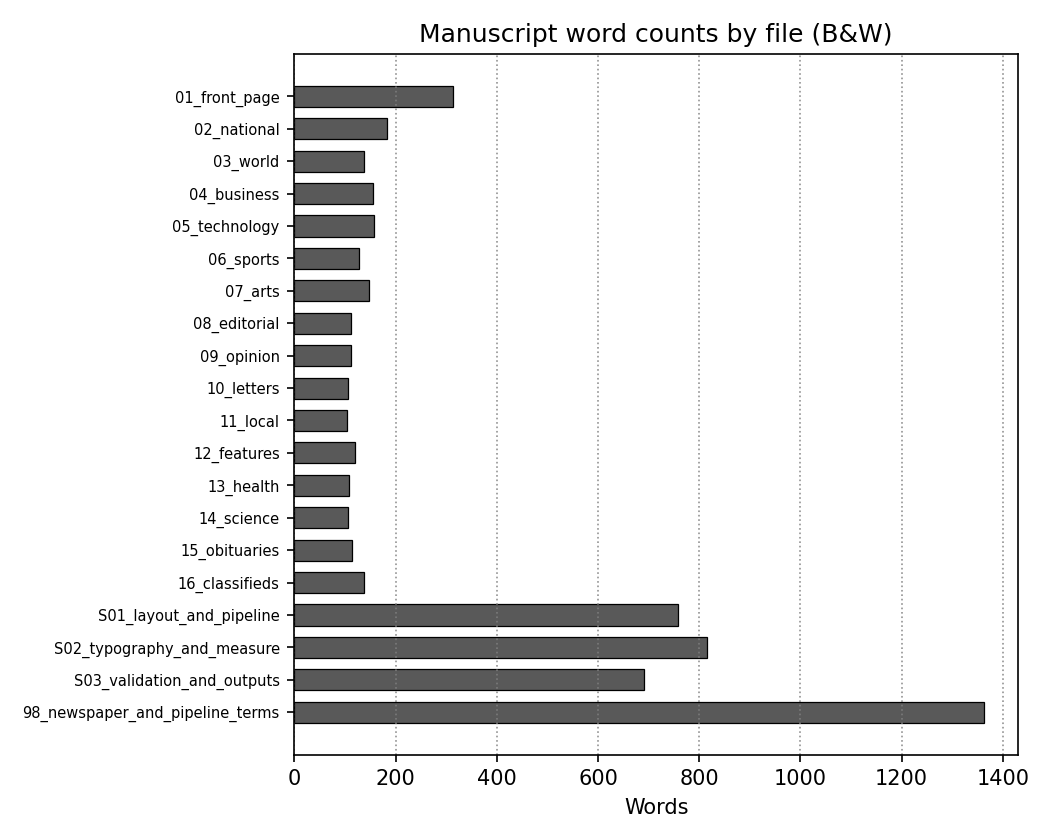
\includegraphics[width=0.92\linewidth]{../figures/wordcount_bars_bw.png}
\caption{Black-and-white horizontal bar chart of word counts per manuscript slice, generated from \texttt{manuscript\_stats.json} by \texttt{visualization\_wordcount\_bw.py} (runs after \texttt{report\_manuscript\_stats.py} in analysis). Bars use grayscale fills only.}
\label{fig:wordcount_bw}
\end{figure}
\begin{multicols}{3}

Figure\textasciitilde{}\ref{fig:wordcount_bw} summarizes edition word
counts for quick sanity checks alongside validators below.

\textbf{Markdown validation.} Run
\texttt{python3\ -m\ infrastructure.validation.cli\ markdown\ projects/traditional\_newspaper/manuscript/}
before large merges. The CLI checks reference integrity, image paths,
and other structural rules configurable per project. Failures should
block PDF generation in CI the same way failing tests do.

\textbf{PDF validation.} After render,
\texttt{python3\ -m\ infrastructure.validation.cli\ pdf\ output/traditional\_newspaper/pdf/}
scans for unresolved citations (\texttt{{[}?{]}}), reference tokens
(\texttt{??}), and common LaTeX warnings surfaced in text extraction.
Treat warnings as debt even when builds succeed.

\textbf{Combined artifact paths.} Combined markdown often lands at
\texttt{output/traditional\_newspaper/pdf/\_combined\_manuscript.md}
during debugging; the compiled PDF is
\texttt{traditional\_newspaper\_combined.pdf} (exact names follow
renderer conventions). Individual section PDFs help bisect errors when
one slice breaks LaTeX.

\textbf{Web output.} \texttt{WebRenderer} produces HTML under
\texttt{output/traditional\_newspaper/web/}. Figures embedded via raw
LaTeX become \texttt{\textless{}figure\textgreater{}} elements when Lua
filters recognize \texttt{\textbackslash{}begin\{figure\}} blocks.
Verify captions render after changing caption text.

\textbf{Slides.} Beamer slides per stem land in
\texttt{output/traditional\_newspaper/slides/}. Slide builds can fail
independently of the combined PDF if a single section includes
incompatible raw TeX---keep slides in CI if your team relies on them.

\textbf{Data outputs.} \texttt{manuscript\_stats.json} tracks word
counts. \texttt{visualization\_wordcount\_bw.py} reads that JSON and
writes \texttt{../figures/wordcount\_bars\_bw.png} (monochrome bar
chart, Figure\textasciitilde{}\ref{fig:wordcount_bw}).

\textbf{Integrity and checksums.} Optional integrity modules hash
outputs for provenance. Steganography tooling (\texttt{secure\_run.sh})
post-processes PDFs without mutating originals; security-focused teams
may enable it.

\textbf{Failure triage order.} When a build breaks, read the LaTeX log
tail, identify the first undefined control sequence or missing file, fix
that, and rebuild. Pandoc errors precede LaTeX errors chronologically in
logs---start at the earliest failure.

\textbf{Environment reproducibility.} Document \texttt{uv} version,
Python version, and TeX distribution in your lab handbook. Container
images in \texttt{infrastructure/docker/} help teammates match
environments without sharing laptops.

\textbf{Cross-project lessons.} Other projects in the monorepo use the
same validation entry points; fixes to shared infrastructure benefit
everyone. File issues upstream when validators misfire on legitimate
markdown patterns.

\textbf{Longer read: operational playbooks.} Treat validation logs like
server logs: keep the last N successful artifacts, timestamp them, and
attach commit SHAs. When a professor or reviewer asks ``which PDF did
you mean?'', the answer should be a git tag plus a CI run ID, not ``the
one on my desktop.'' Copy stages that mirror \texttt{projects/*/output/}
into \texttt{output/*/} exist precisely so deliverable paths stabilize
for that conversation.

\textbf{Bisection tactics.} If combined PDF fails but individual slices
succeed, binary-search which stem introduces the fault by temporarily
moving half the markdown files aside---careful not to break
\texttt{validate\_inventory}---or by compiling partial combined
markdown. Another approach: inspect \texttt{\_combined\_manuscript.tex}
around the error line LaTeX reports.

\textbf{Performance.} Full XeLaTeX passes dominate pipeline time for
large manuscripts. Caching unchanged slices is tempting but risks stale
cross-references; prefer incremental development on single sections via
\texttt{03\_render\_pdf.py} flags when available, then full combined
builds before release.

\textbf{Artifact hygiene.} \texttt{output/} directories are disposable
per project policy, yet humans treat them as precious.
\texttt{.gitignore} keeps binaries out of version control; document
regeneration commands in README so newcomers are not afraid to delete
stale PDFs.

\textbf{Security scanning.} PDFs can embed JavaScript or launch actions;
validators may flag anomalies. Trusted toolchains reduce surprise. Do
not paste untrusted LaTeX from the internet into \texttt{preamble.md}
without review.

\textbf{Accessibility retesting.} When figure captions change, rerun
HTML export and spot-check screen-reader order: does the caption
immediately follow the image in the DOM? Lua filter ordering can affect
results.

\textbf{Localization.} Validation messages from CLIs are English today;
wrapping them for i18n would help global teams. Manuscript content can
be non-English if fonts and hyphenation languages align---validators
should remain locale-agnostic.

\textbf{Contract tests.} \texttt{validate\_inventory} is a contract:
filenames implied by \texttt{sections.py} must exist. Adding optional
supplements requires updating that tuple---treat it like an API semver
bump for downstream stats scripts.

\textbf{Hand-off checklist.} Before declaring a release: all tests
green, markdown validation clean, PDF validation clean, figures
regenerated, \texttt{manuscript\_stats.json} refreshed, and a human
skimmed captions for typos. Automation covers everything except the last
step---for now.

\end{multicols}

\newpage

\section{Glossary: Newspaper and pipeline
terms}\label{glossary-newspaper-and-pipeline-terms}

\begin{figure}[!ht]
\centering

\includegraphics[width=\linewidth]{../figures/section_banner_98_newspaper_and_pipeline_terms.png}
\caption{Glossary folio banner (B\&W).}
\label{fig:banner_glossary}
\end{figure}

Short definitions for readers of this exemplar (not a general journalism
style guide). Terms apply to the \texttt{traditional\_newspaper} project
and the surrounding template infrastructure unless noted.

{\def\LTcaptype{none} % do not increment counter
\begin{longtable}[]{@{}
  >{\raggedright\arraybackslash}p{(\linewidth - 2\tabcolsep) * \real{0.2727}}
  >{\raggedright\arraybackslash}p{(\linewidth - 2\tabcolsep) * \real{0.7273}}@{}}
\toprule\noalign{}
\begin{minipage}[b]{\linewidth}\raggedright
Term
\end{minipage} & \begin{minipage}[b]{\linewidth}\raggedright
Meaning here
\end{minipage} \\
\midrule\noalign{}
\endhead
\bottomrule\noalign{}
\endlastfoot
\textbf{Folio} & One manuscript slice (\texttt{01\_*.md} \ldots{}
\texttt{16\_*.md}) that becomes a new page boundary in the combined PDF
after the previous slice (plus template title front matter). \\
\textbf{Masthead} & The nameplate graphic at the top of the front page;
raster asset \texttt{../figures/masthead.png}, floated and captioned in
the combined PDF (\texttt{fig:masthead}). \\
\textbf{Slice} & Same as folio file: one ordered markdown unit in
\texttt{manuscript/}. \\
\textbf{Preamble} & \texttt{manuscript/preamble.md}: LaTeX injected into
the Pandoc document (geometry, \texttt{graphicx}, \texttt{multicol}). \\
\textbf{Raw LaTeX block} & Pandoc fenced region
\texttt{\textasciigrave{}\textasciigrave{}\textasciigrave{}\{=latex\}}
\ldots{} \texttt{\textasciigrave{}\textasciigrave{}\textasciigrave{}}
passing TeX through to the PDF engine. \\
\textbf{Thin orchestrator} & Script under \texttt{scripts/} that only
configures paths, logging, and calls \texttt{src/newspaper/}
functions. \\
\textbf{Fixture copy} & Deterministic placeholder paragraphs from
\texttt{newspaper.content.fixture\_copy} / \texttt{fixture\_paragraph}
for layout stress tests. \\
\textbf{Figure} & LaTeX \texttt{figure} environment with
\texttt{\textbackslash{}includegraphics},
\texttt{\textbackslash{}caption}, and \texttt{\textbackslash{}label};
autonumbered in PDF, mapped to \texttt{\textless{}figure\textgreater{}}
in HTML when filters match. \\
\textbf{Caption} & Text under a figure explaining content; must avoid
nested \texttt{\}} braces inside \texttt{\textbackslash{}caption\{...\}}
for HTML conversion regexes. \\
\textbf{Label} & \texttt{\textbackslash{}label\{fig:...\}} token paired
with \texttt{\textbackslash{}ref\{...\}} for cross-references resolved
across multiple LaTeX passes. \\
\textbf{Combined PDF} & Single manuscript PDF built from all discovered
slices in order; output path under
\texttt{output/traditional\_newspaper/pdf/}. \\
\textbf{XeLaTeX} & Unicode-capable LaTeX engine used by Pandoc
\texttt{-\/-pdf-engine=xelatex} in this project. \\
\textbf{layout\_schematic.png} & Diagram from
\texttt{render\_layout\_schematic\_png}, written by
\texttt{scripts/generate\_layout\_schematic.py}; illustrates
\texttt{NewspaperLayout} constants. \\
**section\_banner\_*.png** & Wide B\&W header strip per folio (except
the front page), from \texttt{render\_section\_banner\_bw} via
\texttt{scripts/generate\_section\_banners.py}; referenced as
\texttt{fig:banner\_\{stem\}} in markdown. \\
\textbf{PAGE\_SLICES} & Tuple in \texttt{sections.py} mapping stems to
human section titles; defines the sixteen core edition order. \\
\textbf{MANUSCRIPT\_OPTIONAL\_FILENAMES} & Tuple listing \texttt{S01},
\texttt{S02}, \texttt{S03}, and \texttt{98\_*} files included in stats
and documentation beyond core inventory. \\
\textbf{discover\_manuscript\_files} & Infrastructure function sorting
numeric stems, then \texttt{S*}, then \texttt{98\_*}, then
\texttt{99\_*} references. \\
\end{longtable}
}

The sixteen core folios are the ``edition pages'';
\texttt{S01\_*}--\texttt{S03\_*} and \texttt{98\_*} files document the
system without changing the numbering of those pages. When adding
optional slices, extend \texttt{MANUSCRIPT\_OPTIONAL\_FILENAMES} and
update tests that assert file counts.

\subsection{Narrative: how the terms fit
together}\label{narrative-how-the-terms-fit-together}

A \textbf{folio} in this project is both a file and a pagination
boundary. When \texttt{PDFRenderer} concatenates markdown, it inserts
\texttt{\textbackslash{}newpage} between discovered files so each slice
begins a fresh page in the combined document (subject to LaTeX's float
and widow rules). That is looser than historical newspaper ``folio''
usage, which sometimes counted leaves in a signature, but the metaphor
holds: one file, one primary page break intent.

A \textbf{slice} is the same unit under a different metaphor---cutting
the edition into horizontal layers you can reorder only by changing
discovery order or renaming stems. Slices are not nested; there are no
sub-slices inside \texttt{03\_world.md} unless you manually simulate
them with internal headings. Academic papers sometimes use
\texttt{\textbackslash{}section} commands generated by Pandoc; this
project mostly uses markdown headings and raw LaTeX for column wrappers.

The \textbf{preamble} is not a slice. It is metadata injected around the
document skeleton: paper size, packages, hyperref colors, and
\texttt{multicol} parameters. Changing the preamble affects every page,
whereas editing \texttt{11\_local.md} affects only that folio's body
(plus global dependencies like bibliography if you introduce conflicting
packages). Keep preamble changes small and tested; they are the highest
blast-radius edits.

\textbf{Raw LaTeX blocks} are escape hatches. Pandoc's markdown model
does not know about \texttt{multicols} or \texttt{figure} environments,
so this exemplar uses fenced \texttt{\{=latex\}} regions. The cost is
that markdown linters may not analyze inside those fences; LaTeX becomes
the authority. When a build fails, read the TeX log, not just the
markdown validator output.

\textbf{Thin orchestrators} appear under \texttt{scripts/}. They set
\texttt{sys.path}, call \texttt{get\_logger}, invoke one or two
functions from \texttt{src/newspaper/}, and print output paths for
manifest collectors. If you feel tempted to add business logic in a
script, move it into \texttt{src/} and cover it with tests---this
pattern is constitutional for the monorepo.

\textbf{Fixture copy} functions exist so tests can generate paragraphs
without scraping the web. Manuscript prose in this edition is mostly
hand-written now, but \texttt{fixture\_paragraph} remains useful when
generating stress text programmatically or when teaching RNG determinism
with NumPy seeds.

\textbf{Figures}, \textbf{captions}, and \textbf{labels} form a triad.
The float environment owns the visual anchor; the caption explains it;
the label lets prose reference ``Figure 3'' without hard-coding numbers.
HTML export depends on captions being parse-friendly---avoid nested
braces inside \texttt{\textbackslash{}caption\{\}} text because the
conversion filter uses a simple regular expression.

The \textbf{combined PDF} is the integration artifact. Individual slice
PDFs help debugging, but reviewers usually want the stitched book. Paths
vary slightly by renderer configuration; consult
\texttt{output/traditional\_newspaper/pdf/} after a successful run and
look for \texttt{traditional\_newspaper\_combined.pdf} or similarly
named outputs per your local template version.

\textbf{XeLaTeX} handles Unicode font paths better than pdfLaTeX for
many modern workflows. If you switch engines, revisit
\texttt{preamble.md} for font packages and compile twice (or more)
whenever bibliography or references change.

\textbf{layout\_schematic.png} encodes numbers from
\texttt{NewspaperLayout}. When you change \texttt{column\_sep\_in} or
margins, regenerate the PNG and update supplement copy if narrative
descriptions drift from reality. Tests compare bytes for determinism;
visual review confirms semantics.

\textbf{PAGE\_SLICES} is the authoritative order of core news folios.
Git blame it when someone asks why classifieds are last---because the
exemplar models a full edition arc, not because classifieds are
inherently final in all publications.

\textbf{MANUSCRIPT\_OPTIONAL\_FILENAMES} extends stats and documentation
without participating in the sixteen-slice contract. Forgetting to
append a new \texttt{S04} file here means
\texttt{report\_manuscript\_stats.py} might skip it silently aside from
discovery logs---keep the tuple synchronized.

\textbf{discover\_manuscript\_files} is infrastructure shared across
projects. It excludes \texttt{preamble.md}, \texttt{AGENTS.md},
\texttt{README.md}, and config files so documentation can live beside
manuscripts without polluting PDFs. If you add a new non-manuscript
markdown helper, add its basename to the exclude set upstream rather
than hacking per-project filters.

\subsection{Using this glossary in
reviews}\label{using-this-glossary-in-reviews}

When reviewing a pull request that touches
\texttt{traditional\_newspaper}, scan diffs for: stem renames (inventory
tests), preamble edits (global risk), new floats (caption brace safety),
and optional filename list updates (stats drift). Ask whether prose
changes require regenerating figures or refreshing
\texttt{manuscript\_stats.json}. If the answer is yes, include those
artifacts in the same commit series to keep \texttt{main} reproducible.

When onboarding a collaborator, assign reading order: root
\texttt{README}, this glossary, \texttt{S01} supplement, then skim
folios \texttt{01}--\texttt{16} to feel desk tone. Finally open
\texttt{src/newspaper/AGENTS.md} for API tables. That path moves from
product to implementation without drowning newcomers in LaTeX logs on
day one.

\subsection{Future-facing notes}\label{future-facing-notes}

Future maintainers may add \texttt{S04} slices for internationalization
playbooks, \texttt{S05} for CI diagrams, or \texttt{99\_references.md}
if bibliography pages must be explicit. Each addition should update
\texttt{MANUSCRIPT\_OPTIONAL\_FILENAMES}, bump any
\texttt{len(files)\ \textgreater{}=\ N} tests, and document filenames in
\texttt{manuscript/AGENTS.md}. Skipping those steps creates silent drift
where stats JSON omits new prose even though PDFs include it---confusing
anyone automating length gates.

If the edition grows beyond tabloid stress limits, consider splitting
into morning and evening ``editions'' as separate projects under
\texttt{projects/} rather than inflating one \texttt{PAGE\_SLICES} tuple
forever. The template's multi-project mode already lists several
exemplars; cloning the newspaper pattern is cheaper than special-casing
a thirty-slice megafile in discovery code.

Accessibility improvements might add alt text parameters to
figure-generation functions, propagating into matplotlib
\texttt{savefig} metadata and LaTeX \texttt{alt} macros where supported.
That work belongs in \texttt{src/} with tests asserting non-empty
strings for each public figure.

Security improvements might sandbox LaTeX compilation or validate
included graphics are actually PNG/JPEG magic bytes. Those cross into
infrastructure modules shared by all projects; propose changes upstream
rather than forking locally without coordination.

Performance improvements might parallelize slice PDFs where references
are local---careful: global bibliography and cross-slice references
break naive parallelism. The combined build remains the source of truth
until a graph-based planner understands reference edges.

Finally, keep this glossary honest: when terms change meaning after
refactors, edit rows before the next release tag. Outdated glossaries
erode trust faster than outdated jokes on the sports page.



\bibliography{references}
\end{document}
